\documentclass[output=paper]{langscibook}
\ChapterDOI{10.5281/zenodo.10185934}
\title{Introduction to LFG}
\author{Oleg Belyaev\affiliation{Lomonosov Moscow State University, Institute of Linguistics of the Russian Academy of Sciences, and Pushkin State Russian Language Institute}}
\abstract{This chapter provides a general summary of the architecture of LFG. It is mainly focused on describing the two main syntactic levels, c- and f-structure, and the projection architecture used in LFG in general. It also describes the notation for defining the range of possible c-structures and their corresponding f-structures. Core syntactic mechanisms such as structure sharing and X-bar theory are also briefly covered.}

\IfFileExists{../localcommands.tex}{
   \addbibresource{../localbibliography.bib}
   \addbibresource{thisvolume.bib}
   % add all extra packages you need to load to this file

\usepackage{tabularx}
\usepackage{multicol}
\usepackage{url}
\urlstyle{same}
%\usepackage{amsmath,amssymb}

% Tight underlining according to https://alexwlchan.net/2017/10/latex-underlines/
\usepackage{contour}
\usepackage[normalem]{ulem}
\renewcommand{\ULdepth}{1.8pt}
\contourlength{0.8pt}
\newcommand{\tightuline}[1]{%
  \uline{\phantom{#1}}%
  \llap{\contour{white}{#1}}}
  
\usepackage{listings}
\lstset{basicstyle=\ttfamily,tabsize=2,breaklines=true}

% \usepackage{langsci-basic}
\usepackage{langsci-optional}
\usepackage[danger]{langsci-lgr}
\usepackage{langsci-gb4e}
%\usepackage{langsci-linguex}
%\usepackage{langsci-forest-setup}
\usepackage[tikz]{langsci-avm} % added tikz flag, 29 July 21
% \usepackage{langsci-textipa}

\usepackage[linguistics,edges]{forest}
\usepackage{tikz-qtree}
\usetikzlibrary{positioning, tikzmark, arrows.meta, calc, matrix, shapes.symbols}
\usetikzlibrary{arrows, arrows.meta, shapes, chains, decorations.text}

%%%%%%%%%%%%%%%%%%%%% Packages for all chapters

% arrows and lines between structures
\usepackage{pst-node}

% lfg attributes and values, lines (relies on pst-node), lexical entries, phrase structure rules
\usepackage{packages/lfg-abbrevs}

% subfigures
\usepackage{subcaption}

% macros for small illustrations in the glossary
\usepackage{./packages/picins}

%%%%%%%%%%%%%%%%%%%%% Packages from contributors

% % Simpler Syntax packages
\usepackage{bm}
\tikzstyle{block} = [rectangle, draw, text width=5em, text centered, minimum height=3em]
\tikzstyle{line} = [draw, thick, -latex']

% Dependency packages
\usepackage{tikz-dependency}
%\usepackage{sdrt}

\usepackage{soul}

\usepackage[notipa]{ot-tableau}

% Historical
\usepackage{stackengine}
\usepackage{bigdelim}

% Morphology
\usepackage{./packages/prooftree}
\usepackage{arydshln}
\usepackage{stmaryrd}

% TAG
\usepackage{pbox}

\usepackage{langsci-branding}

   % %%%%%%%%% lang sci press commands

\newcommand*{\orcid}{}

\makeatletter
\let\thetitle\@title
\let\theauthor\@author
\makeatother

\newcommand{\togglepaper}[1][0]{
   \bibliography{../localbibliography}
   \papernote{\scriptsize\normalfont
     \theauthor.
     \titleTemp.
     To appear in:
     Dalrymple, Mary (ed.).
     Handbook of Lexical Functional Grammar.
     Berlin: Language Science Press. [preliminary page numbering]
   }
   \pagenumbering{roman}
   \setcounter{chapter}{#1}
   \addtocounter{chapter}{-1}
}

\DeclareOldFontCommand{\rm}{\normalfont\rmfamily}{\mathrm}
\DeclareOldFontCommand{\sf}{\normalfont\sffamily}{\mathsf}
\DeclareOldFontCommand{\tt}{\normalfont\ttfamily}{\mathtt}
\DeclareOldFontCommand{\bf}{\normalfont\bfseries}{\mathbf}
\DeclareOldFontCommand{\it}{\normalfont\itshape}{\mathit}
\makeatletter
\DeclareOldFontCommand{\sc}{\normalfont\scshape}{\@nomath\sc}
\makeatother

% Bug fix, 3 April 2021
\SetupAffiliations{output in groups = false,
                   separator between two = {\bigskip\\},
                   separator between multiple = {\bigskip\\},
                   separator between final two = {\bigskip\\}
                   }

% commands for all chapters
\setmathfont{LibertinusMath-Additions.otf}[range="22B8]

% punctuation between a sequence of years in a citation
% OLD: \renewcommand{\compcitedelim}{\multicitedelim}
\renewcommand{\compcitedelim}{\addcomma\space}

% \citegen with no parentheses around year
\providecommand{\citegenalt}[2][]{\citeauthor{#2}'s \citeyear*[#1]{#2}}

% avms with plain font, using langsci-avm package
\avmdefinestyle{plain}{attributes=\normalfont,values=\normalfont,types=\normalfont,extraskip=0.2em}
% avms with attributes and values in small caps, using langsci-avm package
\avmdefinestyle{fstr}{attributes=\scshape,values=\scshape,extraskip=0.2em}
% avms with attributes in small caps, values in plain font (from peter sells)
\avmdefinestyle{fstr-ps}{attributes=\scshape,values=\normalfont,extraskip=0.2em}

% reference to previous or following examples, from Stefan
%(\mex{1}) is like \next, referring to the next example
%(\mex{0}) is like \last, referring to the previous example, etc
\makeatletter
\newcommand{\mex}[1]{\the\numexpr\c@equation+#1\relax}
\makeatother

% do not add xspace before these
\xspaceaddexceptions{1234=|*\}\restrict\,}

% Several chapters use evnup -- this is verbatim from lingmacros.sty
\makeatletter
\def\evnup{\@ifnextchar[{\@evnup}{\@evnup[0pt]}}
\def\@evnup[#1]#2{\setbox1=\hbox{#2}%
\dimen1=\ht1 \advance\dimen1 by -.5\baselineskip%
\advance\dimen1 by -#1%
\leavevmode\lower\dimen1\box1}
\makeatother

% Centered entries in tables.  Requires array package.
\newcolumntype{P}[1]{>{\centering\arraybackslash}p{#1}}

% Reference to multiple figures, requested by Victoria Rosen
\newcommand{\figsref}[2]{Figures~\ref{#1}~and~\ref{#2}}
\newcommand{\figsrefthree}[3]{Figures~\ref{#1},~\ref{#2}~and~\ref{#3}}
\newcommand{\figsreffour}[4]{Figures~\ref{#1},~\ref{#2},~\ref{#3}~and~\ref{#4}}
\newcommand{\figsreffive}[5]{Figures~\ref{#1},~\ref{#2},~\ref{#3},~\ref{#4}~and~\ref{#5}}

% Semitic chapter:
\providecommand{\textchi}{χ}

% Prosody chapter
\makeatletter
\providecommand{\leftleadsto}{%
  \mathrel{\mathpalette\reflect@squig\relax}%
}
\newcommand{\reflect@squig}[2]{%
  \reflectbox{$\m@th#1$$\leadsto$}%
}
\makeatother
\newcommand\myrotaL[1]{\mathrel{\rotatebox[origin=c]{#1}{$\leadsto$}}}
\newcommand\Prosleftarrow{\myrotaL{-135}}
\newcommand\myrotaR[1]{\mathrel{\rotatebox[origin=c]{#1}{$\leftleadsto$}}}
\newcommand\Prosrightarrow{\myrotaR{135}}

% Core Concepts chapter
\newcommand{\anterm}[2]{#1\\#2}
\newcommand{\annode}[2]{#1\\#2}

% HPSG chapter
\newcommand{\HPSGphon}[1]{〈#1〉}
% for defining RSRL relations:
\newcommand{\HPSGsfl}{\enskip\ensuremath{\stackrel{\forall{}}{\Longleftarrow{}}}\enskip}
% AVM commands, valid only inside \avm{}
\avmdefinecommand {phon}[phon] { attributes=\itshape } % define a new \phon command
% Forest Set-up
\forestset
  {notin label above/.style={edge label={node[midway,sloped,above,inner sep=0pt]{\strut$\ni$}}},
    notin label below/.style={edge label={node[midway,sloped,below,inner sep=0pt]{\strut$\ni$}}},
  }

% Dependency chapter
\newcommand{\ua}{\ensuremath{\uparrow}}
\newcommand{\da}{\ensuremath{\downarrow}}
\forestset{
  dg edges/.style={for tree={parent anchor=south, child anchor=north,align=center,base=bottom},
                 where n children=0{tier=word,edge=dotted,calign with current edge}{}
                },
dg transfer/.style={edge path={\noexpand\path[\forestoption{edge}, rounded corners=3pt]
    % the line downwards
    (!u.parent anchor)-- +($(0,-l)-(0,4pt)$)-- +($(12pt,-l)-(0,4pt)$)
    % the horizontal line
    ($(!p.north west)+(0,l)-(0,20pt)$)--($(.north east)+(0,l)-(0,20pt)$)\forestoption{edge label};},!p.edge'={}},
% for Tesniere-style junctions
dg junction/.style={no edge, tikz+={\draw (!p.east)--(!.west) (.east)--(!n.west);}    }
}


% Glossary
\makeatletter % does not work with \newcommand
\def\namedlabel#1#2{\begingroup
   \def\@currentlabel{#2}%
   \phantomsection\label{#1}\endgroup
}
\makeatother


\renewcommand{\textopeno}{ɔ}
\providecommand{\textepsilon}{ɛ}

\renewcommand{\textbari}{ɨ}
\renewcommand{\textbaru}{ʉ}
\newcommand{\acutetextbari}{í̵}
\renewcommand{\textlyoghlig}{ɮ}
\renewcommand{\textdyoghlig}{ʤ}
\renewcommand{\textschwa}{ə}
\renewcommand{\textprimstress}{ˈ}
\newcommand{\texteng}{ŋ}
\renewcommand{\textbeltl}{ɬ}
\newcommand{\textramshorns}{ɤ}

\newbool{bookcompile}
\booltrue{bookcompile}
\newcommand{\bookorchapter}[2]{\ifbool{bookcompile}{#1}{#2}}




\renewcommand{\textsci}{ɪ}
\renewcommand{\textturnscripta}{ɒ}

\renewcommand{\textscripta}{ɑ}
\renewcommand{\textteshlig}{ʧ}
\providecommand{\textupsilon}{υ}
\renewcommand{\textyogh}{ʒ}
\newcommand{\textpolhook}{̨}

\renewcommand{\sectref}[1]{Section~\ref{#1}}

%\KOMAoptions{chapterprefix=true}

\renewcommand{\textturnv}{ʌ}
\renewcommand{\textrevepsilon}{ɜ}
\renewcommand{\textsecstress}{ˌ}
\renewcommand{\textscriptv}{ʋ}
\renewcommand{\textglotstop}{ʔ}
\renewcommand{\textrevglotstop}{ʕ}
%\newcommand{\textcrh}{ħ}
\renewcommand{\textesh}{ʃ}

% label for submitted and published chapters
\newcommand{\submitted}{{\color{red}Final version submitted to Language Science Press.}}
\newcommand{\published}{{\color{red}Final version published by
    Language Science Press, available at \url{https://langsci-press.org/catalog/book/312}.}}

% Treebank definitions
\definecolor{tomato}{rgb}{0.9,0,0}
\definecolor{kelly}{rgb}{0,0.65,0}

% Minimalism chapter
\newcommand\tr[1]{$<$\textcolor{gray}{#1}$>$}
\newcommand\gapline{\lower.1ex\hbox to 1.2em{\bf \ \hrulefill\ }}
\newcommand\cnom{{\llap{[}}Case:Nom{\rlap{]}}}
\newcommand\cacc{{\llap{[}}Case:Acc{\rlap{]}}}
\newcommand\tpres{{\llap{[}}Tns:Pres{\rlap{]}}}
\newcommand\fstackwe{{\llap{[}}Tns:Pres{\rlap{]}}\\{\llap{[}}Pers:1{\rlap{]}}\\{\llap{[}}Num:Pl{\rlap{]}}}
\newcommand\fstackone{{\llap{[}}Tns:Past{\rlap{]}}\\{\llap{[}}Pers:\ {\rlap{]}}\\{\llap{[}}Num:\ {\rlap{]}}}
\newcommand\fstacktwo{{\llap{[}}Pers:3{\rlap{]}}\\{\llap{[}}Num:Pl{\rlap{]}}\\{\llap{[}}Case:\ {\rlap{]}}}
\newcommand\fstackthr{{\llap{[}}Tns:Past{\rlap{]}}\\{\llap{[}}Pers:3{\rlap{]}}\\{\llap{[}}Num:Pl{\rlap{]}}} 
\newcommand\fstackfou{{\llap{[}}Pers:3{\rlap{]}}\\{\llap{[}}Num:Pl{\rlap{]}}\\{\llap{[}}Case:Nom{\rlap{]}}}
\newcommand\fstackonefill{{\llap{[}}Tns:Past{\rlap{]}}\\{\llap{[}}Pers:3{\rlap{]}}\\%
  {\llap{[}}Num:Pl{\rlap{]}}}
\newcommand\fstackoneint%
    {{\llap{[}}{\bf Tns:Past}{\rlap{]}}\\{\llap{[}}Pers:\ {\rlap{]}}\\{\llap{[}}Num:\ {\rlap{]}}}
\newcommand\fstacktwoint%
    {{\llap{[}}{\bf Pers:3}{\rlap{]}}\\{\llap{[}}{\bf Num:Pl}{\rlap{]}}\\{\llap{[}}Case:\ {\rlap{]}}}
\newcommand\fstackthrchk%
    {{\llap{[}}{\bf Tns:Past}{\rlap{]}}\\{\llap{[}}{Pers:3}{\rlap{]}}\\%
      {\llap{[}}Num:Pl{\rlap{]}}} 
\newcommand\fstackfouchk%
    {{\llap{[}}{\bf Pers:3}{\rlap{]}}\\{\llap{[}}{\bf Num:Pl}{\rlap{]}}\\%
      {\llap{[}}Case:Nom{\rlap{]}}}
\newcommand\uinfl{{\llap{[}}Infl:\ \ {\rlap{]}}}
\newcommand\inflpass{{\llap{[}}Infl:Pass{\rlap{]}}}
\newcommand\fepp{{\llap{[}}EPP{\rlap{]}}}
\newcommand\sepp{{\llap{[}}\st{EPP}{\rlap{]}}}
\newcommand\rdash{\rlap{\hbox to 24em{\hfill (dashed lines represent
      information flow)}}}


% Computational chapter
\usepackage{./packages/kaplan}
\renewcommand{\red}{\color{lsLightWine}}

% Sinitic
\newcommand{\FRAME}{\textsc{frame}\xspace}
\newcommand{\arglistit}[1]{{\textlangle}\textit{#1}{\textrangle}}

%WestGermanic
\newcommand{\streep}[1]{\mbox{\rule{1pt}{0pt}\rule[.5ex]{#1}{.5pt}\rule{-1pt}{0pt}\rule{-#1}{0pt}}}

\newcommand{\hspaceThis}[1]{\hphantom{#1}}


\newcommand{\FIG}{\textsc{figure}}
\newcommand{\GR}{\textsc{ground}}

%%%%% Morphology
% Single quote
\newcommand{\asquote}[1]{`{#1}'} % Single quotes
\newcommand{\atrns}[1]{\asquote{#1}} % Translation
\newcommand{\attrns}[1]{(\asquote{#1})} % Translation
\newcommand{\ascare}[1]{\asquote{#1}} % Scare quotes
\newcommand{\aqterm}[1]{\asquote{#1}} % Quoted terms
% Double quote
\newcommand{\adquote}[1]{``{#1}''} % Double quotes
\newcommand{\aquoot}[1]{\adquote{#1}} % Quotes
% Italics
\newcommand{\aword}[1]{\textit{#1}}  % mention of word
\newcommand{\aterm}[1]{\textit{#1}}
% Small caps
\newcommand{\amg}[1]{{\textsc{\MakeLowercase{#1}}}}
\newcommand{\ali}[1]{\MakeLowercase{\textsc{#1}}}
\newcommand{\feat}[1]{{\textsc{#1}}}
\newcommand{\val}[1]{\textsc{#1}}
\newcommand{\pred}[1]{\textsc{#1}}
\newcommand{\predvall}[1]{\textsc{#1}}
% Misc commands
\newcommand{\exrr}[2][]{(\ref{ex:#2}{#1})}
\newcommand{\csn}[3][t]{\begin{tabular}[#1]{@{\strut}c@{\strut}}#2\\#3\end{tabular}}
\newcommand{\sem}[2][]{\ensuremath{\left\llbracket \mbox{#2} \right\rrbracket^{#1}}}
\newcommand{\apf}[2][\ensuremath{\sigma}]{\ensuremath{\langle}#2,#1\ensuremath{\rangle}}
\newcommand{\formula}[2][t]{\ensuremath{\begin{array}[#1]{@{\strut}l@{\strut}}#2%
                                         \end{array}}}
\newcommand{\Down}{$\downarrow$}
\newcommand{\Up}{$\uparrow$}
\newcommand{\updown}{$\uparrow=\downarrow$}
\newcommand{\upsigb}{\mbox{\ensuremath{\uparrow\hspace{-0.35em}_\sigma}}}
\newcommand{\lrfg}{L\textsubscript{R}FG} 
\newcommand{\dmroot}{\ensuremath{\sqrt{\hspace{1em}}}}
\newcommand{\amother}{\mbox{\ensuremath{\hat{\raisebox{-.25ex}{\ensuremath{\ast}}}}}}
\newcommand{\expone}{\ensuremath{\xrightarrow{\nu}}}
\newcommand{\sig}{\mbox{$_\sigma\,$}}
\newcommand{\aset}[1]{\{#1\}}
\newcommand{\linimp}{\mbox{\ensuremath{\,\multimap\,}}}
\newcommand{\fsfunc}{\ensuremath{\Phi}\hspace*{-.15em}}
\newcommand{\cons}[1]{\ensuremath{\mbox{\textbf{\textup{#1}}}}}
\newcommand{\amic}[1][]{\cons{MostInformative$_c$}{#1}}
\newcommand{\amif}[1][]{\cons{MostInformative$_f$}{#1}}
\newcommand{\amis}[1][]{\cons{MostInformative$_s$}{#1}}
\newcommand{\amsp}[1][]{\cons{MostSpecific}{#1}}

%Glue
\newcommand{\glues}{Glue Semantics} % macro for consistency
\newcommand{\glue}{Glue} % macro for consistency
\newcommand{\lfgglue}{LFG$+$Glue} 
\newcommand{\scare}[1]{`{#1}'} % Scare quotes
\newcommand{\word}[1]{\textit{#1}}  % mention of word
\newcommand{\dquote}[1]{``{#1}''} % Double quotes
\newcommand{\high}[1]{\textit{#1}} % highlight (italicize)
\newcommand{\laml}{{L}} 
% Left interpretation double bracket
\newcommand{\Lsem}{\ensuremath{\left\llbracket}} 
% Right interpretation double bracket
\newcommand{\Rsem}{\ensuremath{\right\rrbracket}} 
\newcommand{\nohigh}[1]{{#1}} % nohighlight (regular font)
% Linear implication elimination
\newcommand{\linimpE}{\mbox{\small\ensuremath{\multimap_{\mathcal{E}}}}}
% Linear implication introduction, plain
\newcommand{\linimpI}{\mbox{\small\ensuremath{\multimap_{\mathcal{I}}}}}
% Linear implication introduction, with flag
\newcommand{\linimpIi}[1]{\mbox{\small\ensuremath{\multimap_{{\mathcal{I}},#1}}}}
% Linear universal elimination
\newcommand{\forallE}{\mbox{\small\ensuremath{\forall_{{\mathcal{E}}}}}}
% Tensor elimination
\newcommand{\tensorEij}[2]{\mbox{\small\ensuremath{\otimes_{{\mathcal{E}},#1,#2}}}}
% CG forward slash
\newcommand{\fs}{\ensuremath{/}} 
% s-structure mapping, no space after                                     
\newcommand{\sigb}{\mbox{$_\sigma$}}
% uparrow with s-structure mapping, with small space after  
\newcommand{\upsig}{\mbox{\ensuremath{\uparrow\hspace{-0.35em}_\sigma\,}}}
\newcommand{\fsa}[1]{\textit{#1}}
\newcommand{\sqz}[1]{#1}
% Angled brackets (types, etc.)
\newcommand{\bracket}[1]{\ensuremath{\left\langle\mbox{\textit{#1}}\right\rangle}}
% glue logic string term
\newcommand{\gterm}[1]{\ensuremath{\mbox{\textup{\textit{#1}}}}}
% abstract grammatical formative
\newcommand{\gform}[1]{\ensuremath{\mbox{\textsc{\textup{#1}}}}}
% let
\newcommand{\llet}[3]{\ensuremath{\mbox{\textsf{let}}~{#1}~\mbox{\textsf{be}}~{#2}~\mbox{\textsf{in}}~{#3}}}
% Word-adorned proof steps
\providecommand{\vformula}[2]{%
  \begin{array}[b]{l}
    \mbox{\textbf{\textit{#1}}}\\%[-0.5ex]
    \formula{#2}
  \end{array}
}

%TAG
\newcommand{\fm}[1]{\textsc{#1}}
\newcommand{\struc}[1]{{#1-struc\-ture}}
\newcommand{\func}[1]{\mbox{#1-function}}
\newcommand{\fstruc}{\struc{f}}
\newcommand{\cstruc}{\struc{c}}
\newcommand{\sstruc}{\struc{s}}
\newcommand{\astruc}{\struc{a}}
\newcommand{\nodelabels}[2]{\rlap{\ensuremath{^{#1}_{#2}}}}
\newcommand{\footnode}{\rlap{\ensuremath{^{*}}}}
\newcommand{\nafootnode}{\rlap{\ensuremath{^{*}_{\nalabel}}}}
\newcommand{\nanode}{\rlap{\ensuremath{_{\nalabel}}}}
\newcommand{\AdjConstrText}[1]{\textnormal{\small #1}}
\newcommand{\nalabel}{\AdjConstrText{NA}}

%Case
\newcommand{\MID}{\textsc{mid}{}\xspace}

%font commands added April 2023 for Control and Case chapters
\def\textthorn{þ}
\def\texteth{ð}
\def\textinvscr{ʁ}
\def\textcrh{ħ}
\def\textgamma{ɣ}

% Coordination
\newcommand{\CONJ}{\textsc{conj}{}\xspace}
\newcommand*{\phtm}[1]{\setbox0=\hbox{#1}\hspace{\wd0}}
\newcommand{\ggl}{\hfill(Google)}
\newcommand{\nkjp}{\hfill(NKJP)}

% LDDs
\newcommand{\ubd}{\attr{ubd}\xspace}
% \newcommand{\disattr}[1]{\blue \attr{#1}}  % on topic/focus path
% \newcommand{\proattr}[1]{\green\attr{#1}}  % On Q/Relpro path
\newcommand{\disattr}[1]{\color{lsMidBlue}\attr{#1}}  % on topic/focus path
\newcommand{\proattr}[1]{\color{lsMidGreen}\attr{#1}}  % On Q/Relpro path
\newcommand{\eestring}{\mbox{$e$}\xspace}
\providecommand{\disj}[1]{\{\attr{#1}\}}
\providecommand{\estring}{\mb{\epsilon}}
\providecommand{\termcomp}[1]{\attr{\backslash {#1}}}
\newcommand{\templatecall}[2]{{\small @}(\attr{#1}\ \attr{#2})}
\newcommand{\xlgf}[1]{(\leftarrow\ \attr{#1})} 
\newcommand{\xrgf}[1]{(\rightarrow\ \attr{#1})}
\newcommand{\rval}[2]{\annobox {\xrgf{#1}\teq\attr{#2}}}
\newcommand{\memb}[1]{\annobox {\downarrow\, \in \xugf{#1}}}
\newcommand{\lgf}[1]{\annobox {\xlgf{#1}}}
\newcommand{\rgf}[1]{\annobox {\xrgf{#1}}}
\newcommand{\rvalc}[2]{\annobox {\xrgf{#1}\teqc\attr{#2}}}
\newcommand{\xgfu}[1]{(\attr{#1}\uparrow)}
\newcommand{\gfu}[1]{\annobox {\xgfu{#1}}}
\newcommand{\nmemb}[3]{\annobox {{#1}\, \in \ngf{#2}{#3}}}
\newcommand{\dgf}[1]{\annobox {\xdgf{#1}}}
\newcommand{\predsfraise}[3]{\annobox {\xugf{pred}\teq\semformraise{#1}{#2}{#3}}}
\newcommand{\semformraise}[3]{\annobox {\textrm{`}\hspace{-.05em}\attr{#1}\langle\attr{#2}\rangle{\attr{#3}}\textrm{'}}}
\newcommand{\teqc}{\hspace{-.1667em}=_c\hspace{-.1667em}} 
\newcommand{\lval}[2]{\annobox {\xlgf{#1}\teq\attr{#2}}}
\newcommand{\xgfd}[1]{(\attr{#1}\downarrow)}
\newcommand{\gfd}[1]{\annobox {\xgfd{#1}}}
\newcommand{\gap}{\rule{.75em}{.5pt}\ }
\newcommand{\gapp}{\rule{.75em}{.5pt}$_p$\ }

% Mapping
% Avoid having to write 'argument structure' a million times
\newcommand{\argstruc}{argument structure}
\newcommand{\Argstruc}{Argument structure}
\newcommand{\emptybracks}{\ensuremath{[\;\;]}}
\newcommand{\emptycurlybracks}{\ensuremath{\{\;\;\}}}
% Drawing lines in structures
\newcommand{\strucconnect}[6]{%
\draw[-stealth] (#1) to[out=#5, in=#6] node[pos=#3, above]{#4} (#2);%
}
\newcommand{\strucconnectdashed}[6]{%
\draw[-stealth, dashed] (#1) to[out=#5, in=#6] node[pos=#3, above]{#4} (#2);%
}
% Attributes for s-structures in the style of lfg-abbrevs.sty
\newcommand{\ARGnum}[1]{\textsc{arg}\textsubscript{#1}}
% Drawing mapping lines
\newcommand{\maplink}[2]{%
\begin{tikzpicture}[baseline=(A.base)]
\node(A){#1\strut};
\node[below = 3ex of A](B){\pbox{\textwidth}{#2}};
\draw ([yshift=-1ex]A.base)--(B);
% \draw (A)--(B);
\end{tikzpicture}}
% long line for extra features
\newcommand{\longmaplink}[2]{%
\begin{tikzpicture}[baseline=(A.base)]
\node(A){#1\strut};
\node[below = 3ex of A](B){\pbox{\textwidth}{#2}};
\draw ([yshift=2.5ex]A.base)--(B);
% \draw (A)--(B);
\end{tikzpicture}%
}
% For drawing upward
\newcommand{\maplinkup}[2]{%
\begin{tikzpicture}[baseline=(A.base)]
\node(A){#1};
\node[above = 3ex of A, anchor=base](B){#2};
\draw (A)--(B);
\end{tikzpicture}}
% Above with arrow going down (for argument adding processes)
\newcommand{\argumentadd}[2]{%
\begin{tikzpicture}[baseline=(A.base)]
\node(A){#1};
\node[above = 3ex of A, anchor=base](B){#2};
\draw[latex-] ([yshift=2ex]A.base)--([yshift=-1ex]B.center);
\end{tikzpicture}}
% Going up to the left
\newcommand{\maplinkupleft}[2]{%
\begin{tikzpicture}[baseline=(A.base)]
\node(A){#1};
\node[above left = 3ex of A, anchor=base](B){#2};
\draw (A)--(B);
\end{tikzpicture}}
% Going up to the right
\newcommand{\maplinkupright}[2]{%
\begin{tikzpicture}[baseline=(A.base)]
\node(A){#1};
\node[above right = 3ex of A, anchor=base](B){#2};
\draw (A)--(B);
\end{tikzpicture}}
% Argument fusion
\newenvironment{tikzsentence}{\begin{tikzpicture}[baseline=0pt, 
  anchor=base, outer sep=0pt, ampersand replacement=\&
   ]}{\end{tikzpicture}}
\newcommand{\Subnode}[2]{\subnode[inner sep=1pt]{#1}{#2\strut}}
\newcommand{\connectbelow}[3]{\draw[inner sep=0pt] ([yshift=0.5ex]#1.south) -- ++ (south:#3ex)
  -| ([yshift=0.5ex]#2.south);}
\newcommand{\connectabove}[3]{\draw[inner sep=0pt] ([yshift=0ex]#1.north) -- ++ (north:#3ex)
  -| ([yshift=0ex]#2.north);}
  
\newcommand{\ASNode}[2]{\tikz[remember picture,baseline=(#1.base)] \node [anchor=base] (#1) {#2};}

% Austronesian
\newcommand{\LV}{\textsc{lv}\xspace}
\newcommand{\IV}{\textsc{iv}\xspace}
\newcommand{\DV}{\textsc{dv}\xspace}
\newcommand{\PV}{\textsc{pv}\xspace}
\newcommand{\AV}{\textsc{av}\xspace}
\newcommand{\UV}{\textsc{uv}\xspace}

\apptocmd{\appendix}
         {\bookmarksetup{startatroot}}
         {}
         {%
           \AtEndDocument{\typeout{langscibook Warning:}
                          \typeout{It was not possible to set option 'staratroot'}
                          \typeout{for appendix in the backmatter.}}
         }

   %% hyphenation points for line breaks
%% Normally, automatic hyphenation in LaTeX is very good
%% If a word is mis-hyphenated, add it to this file
%%
%% add information to TeX file before \begin{document} with:
%% %% hyphenation points for line breaks
%% Normally, automatic hyphenation in LaTeX is very good
%% If a word is mis-hyphenated, add it to this file
%%
%% add information to TeX file before \begin{document} with:
%% %% hyphenation points for line breaks
%% Normally, automatic hyphenation in LaTeX is very good
%% If a word is mis-hyphenated, add it to this file
%%
%% add information to TeX file before \begin{document} with:
%% \include{localhyphenation}
\hyphenation{
Aus-tin
Bel-ya-ev
Bres-nan
Chom-sky
Eng-lish
Geo-Gram
INESS
Inkelas
Kaplan
Kok-ko-ni-dis
Lacz-kó
Lam-ping
Lu-ra-ghi
Lund-quist
Mcho-mbo
Meu-rer
Nord-lin-ger
PASSIVE
Pa-no-va
Pol-lard
Pro-sod-ic
Prze-piór-kow-ski
Ram-chand
Sa-mo-ye-dic
Tsu-no-da
WCCFL
Wam-ba-ya
Warl-pi-ri
Wes-coat
Wo-lof
Zae-nen
accord-ing
an-a-phor-ic
ana-phor
christ-church
co-description
co-present
con-figur-ation-al
in-effa-bil-ity
mor-phe-mic
mor-pheme
non-com-po-si-tion-al
pros-o-dy
referanse-grammatikk
rep-re-sent
Schätz-le
term-hood
Kip-ar-sky
Kok-ko-ni
Chi-che-\^wa
au-ton-o-mous
Al-si-na
Ma-tsu-mo-to
}

\hyphenation{
Aus-tin
Bel-ya-ev
Bres-nan
Chom-sky
Eng-lish
Geo-Gram
INESS
Inkelas
Kaplan
Kok-ko-ni-dis
Lacz-kó
Lam-ping
Lu-ra-ghi
Lund-quist
Mcho-mbo
Meu-rer
Nord-lin-ger
PASSIVE
Pa-no-va
Pol-lard
Pro-sod-ic
Prze-piór-kow-ski
Ram-chand
Sa-mo-ye-dic
Tsu-no-da
WCCFL
Wam-ba-ya
Warl-pi-ri
Wes-coat
Wo-lof
Zae-nen
accord-ing
an-a-phor-ic
ana-phor
christ-church
co-description
co-present
con-figur-ation-al
in-effa-bil-ity
mor-phe-mic
mor-pheme
non-com-po-si-tion-al
pros-o-dy
referanse-grammatikk
rep-re-sent
Schätz-le
term-hood
Kip-ar-sky
Kok-ko-ni
Chi-che-\^wa
au-ton-o-mous
Al-si-na
Ma-tsu-mo-to
}

\hyphenation{
Aus-tin
Bel-ya-ev
Bres-nan
Chom-sky
Eng-lish
Geo-Gram
INESS
Inkelas
Kaplan
Kok-ko-ni-dis
Lacz-kó
Lam-ping
Lu-ra-ghi
Lund-quist
Mcho-mbo
Meu-rer
Nord-lin-ger
PASSIVE
Pa-no-va
Pol-lard
Pro-sod-ic
Prze-piór-kow-ski
Ram-chand
Sa-mo-ye-dic
Tsu-no-da
WCCFL
Wam-ba-ya
Warl-pi-ri
Wes-coat
Wo-lof
Zae-nen
accord-ing
an-a-phor-ic
ana-phor
christ-church
co-description
co-present
con-figur-ation-al
in-effa-bil-ity
mor-phe-mic
mor-pheme
non-com-po-si-tion-al
pros-o-dy
referanse-grammatikk
rep-re-sent
Schätz-le
term-hood
Kip-ar-sky
Kok-ko-ni
Chi-che-\^wa
au-ton-o-mous
Al-si-na
Ma-tsu-mo-to
}

   \togglepaper[1]%%chapternumber
}{}

\newcommand\opn[1]{#1}

\begin{document}
\maketitle
\label{chap:Intro}

\section{Introduction}
 
In this chapter, I aim to summarize the main syntactic levels of LFG, constituent structure (c-structure) and functional structure (f-structure), while providing a general overview of the foundational features of this framework. In \sectref{sect:intro:basic}, I briefly describe the basic architecture of LFG and the overall role played by each of the syntactic levels. In \sectref{sect:intro:c-structure}, I describe the c-structure model used in standard LFG, its understanding of constituency, and the role of X$'$ theory. In \sectref{sect:intro:f-structure}, the notion of f-structure is introduced, together with notational conventions and a system of mapping c-structure to f-structure. In \sectref{sect:intro:addlevels}, I show how the basic system of c- and f-structure can be extended to include other levels of projection that comprise the architecture of LFG.
 
 \section{The basic architecture of LFG\label{sect:intro:basic}}
 
 At the core of LFG architecture as it was originally proposed in \textcite{kaplanbresnan82} is the split of syntax into two levels: constituent structure, or \textbf{c-structure}, and functional structure, or \textbf{f-structure}. The correspondence function $\phi(x)$ maps every c-structure node to an f-structure. As an example, consider the LFG analysis of the sentence \textit{John has seen David} in (\ref{ex:intro:mapping}), where the mapping function is represented by the arrows.
 
 \begin{exe}
 \ex\label{ex:intro:mapping}
   \begin{tabular}[t]{c@{\hspace*{4em}}c}
   \begin{forest}
    [\rnode{ip}{IP}
      [\rnode{np1}{NP}
	[\rnode{n1}{N}
	  [John]
	]
      ]
      [\rnode{ibar}{I$'$}
	[\rnode{i}{I}
	  [has]
	]
	[\rnode{vp}{VP}
	  [\rnode{v}{V}
	    [seen]
	  ]
	  [\rnode{np2}{NP}
	    [\rnode{n2}{N}
	      [David]
	    ]
	  ]
	]
      ]
    ]
    \end{forest} &
   \avm[style=fstr]{\id{f}{\rnode{f}{[
        pred & `see\arglist{($f$ \textsc{subj}) ($f$ \textsc{obj})}'\\
        tense & prs\\
        aspect & perf\\
        subj & \id{g}{\rnode{g}{[ pred & {`John'}\\
                                           pers & 3\\
                                           num & sg\\
                                        ]}}\smallskip\\
        obj & \id{h}{\rnode{h}{[ pred & {`David'}\\
                                                  pers & 3\\
                                                  num & sg\\
                                                ]}}
    ]}}}
    \end{tabular}
\end{exe}
    \nccurve[nodesepA=2pt,nodesepB=0pt,angleA={0},angleB={180},linewidth=.5pt,linecolor=lsRichGreen]{->}{ip}{f}
    \nccurve[nodesepA=2pt,nodesepB=0pt,angleA={0},angleB={180},linewidth=.5pt,linecolor=lsRichGreen]{->}{ibar}{f}
    \nccurve[nodesepA=2pt,nodesepB=0pt,angleA={0},angleB={180},linewidth=.5pt,linecolor=lsRichGreen]{->}{i}{f}
    \nccurve[nodesepA=2pt,nodesepB=0pt,angleA={0},angleB={180},linewidth=.5pt,linecolor=lsRichGreen]{->}{vp}{f}
    \nccurve[nodesepA=2pt,nodesepB=0pt,angleA={0},angleB={180},linewidth=.5pt,linecolor=lsRichGreen]{->}{v}{f}
    %
    \nccurve[nodesepA=2pt,nodesepB=0pt,angleA={0},angleB={190},linewidth=.5pt,linecolor=lsRed]{->}{np1}{g}
    \nccurve[nodesepA=2pt,nodesepB=0pt,angleA={0},angleB={190},linewidth=.5pt,linecolor=lsRed]{->}{n1}{g}
    %
    \nccurve[nodesepA=2pt,nodesepB=0pt,angleA={0},angleB={180},linewidth=.5pt,linecolor=lsMidBlue]{->}{np2}{h}
    \nccurve[nodesepA=2pt,nodesepB=0pt,angleA={0},angleB={180},linewidth=.5pt,linecolor=lsMidBlue]{->}{n2}{h}
    As seen in (\ref{ex:intro:mapping}), the two parallel structures are substantially different: c-structure is a phrase structure tree that represents word order and hierarchical embedding, while f-structure is a feature-value structure that represents predicate-argument relations and the grammatical features of all the major parts of the sentence. Features appear as atomic values of f-structure attributes, while arguments and adjuncts appear as f-structures embedded as values of attributes such as \textsc{subj} and \textsc{obj} in (\ref{ex:intro:mapping}); which arguments can and, indeed, have to appear in the f-structure is specified in the value of the \textsc{pred} attribute. While the mapping between the two structures follows certain constraints imposed both by the formal metalanguage and theoretical considerations (on which see \citetv{chapters/CoreConcepts} and \citetv{chapters/Cstr}, it is, in principle, language-specific: an LFG grammar consists of a set of rules and lexical entries that define the possible c-structures and their corresponding f-structures for a particular language.

    This flexibility in the c- to f-structure correspondence ensures that each corresponds to a particular set of grammatical generalizations. Overall, f-structure is the main syntactic level that represents the predicates, their valencies and grammatical relations, as well as grammatical features such as number, case, aspect and gender. The majority of syntactic phenomena that have to do with feature assignment and feature checking are described using f-structure constraints; these include:

    \begin{itemize}
     \item feature government (case assignment, mood, constraints on the use of non-finite forms, etc.);
     \item agreement;
     \item anaphoric constraints;
     \item wh-movement, topicalization and other long-distance dependencies.
    \end{itemize}
All generalizations that have to do with argument relations and grammatical features have to be stated in terms of f-structure. For instance, a constraint that requires the verb to agree with Spec,IP or to assign accusative case to Comp,VP would be complex and somewhat unnatural to formulate (although not impossible). It is much more simple and natural in LFG for such rules to refer to grammatical functions such as \textsc{subj} and \textsc{obj} instead. This implies that the role of constituent structure is more restricted than in other frameworks; for the most part, c-structure constraints only capture generalizations related to word order and various embedding possibilities.
    
    The correspondence architecture is not limited to syntax. Other projections that map c-structure nodes or f-structures to other structures (such as information structure, semantic structure, or prosody) have been proposed in the literature: see \sectref{sect:intro:addlevels} for details.
 
 \section{C-structure\label{sect:intro:c-structure}}
 
 \subsection{The notion of c-structure}
 
 C-structure (constituent structure) in LFG is a phrase structure tree. Possible trees are defined by a set of context-free statements (``phrase structure rules'') of the type $A\, →\, \alpha$, where $A$ is a nonterminal symbol (representing some syntactic category), while $\alpha$ is a string of nonterminals or a single terminal. A simple set of rules that licenses  the English sentence in (\ref{ex:intro:mapping}) is given in (\ref{ex:intro:psr}). 
 
 \ea\label{ex:intro:psr}
 \begin{tabular}[t]{llll}
 a. IP → NP ~ I$'$ & b. I$'$ → I ~ VP & c. VP → V ~ NP & d. NP → N
 \end{tabular}
 \z
 
 Such rules are well-established in modern linguistics since at least \textcite{chomsky1957syntactic} and so hardly require further discussion. It should however be observed that, in LFG, these should not be understood as ``rules'' in the direct (procedural) sense, but rather a set of phrase structure principles that constrain hierarchical relations between mothers and daughters -- crucially, not between levels further apart, such as granddaughters etc. Phrase structure grammars are one way of describing such principles that has proved most popular among LFG practitioners, but not the only way -- possible alternatives are ID/LP rules \parencite{falk1983} and the specification language described in \textcite{potts2002}, which builds on the specification language in \textcite{blackburn1995a-specification}.
 
 The structures that are constrained in this way are not just strings,\footnote{In fact, in the original version of LFG architecture introduced in \textcite{kapl:89}, c-structure is itself a projection from the string. In recent LFG work, this idea has been developed in more detail by distinguishing between the \textit{s-string} (the string of syntactic units) and the \textit{p-string} (the string of phonological units), see \textcite{DM11} and \citetv{chapters/Prosody} for more information.} but constituent structure trees whose nodes are individually mapped to f-structures, as shown in (\ref{ex:intro:mapping}).
 
 The syntax of phrase structure rules in LFG is somewhat more extensive than in many other frameworks, because the right-hand side $\alpha$ is allowed to be a regular expression and include such features as optionality (represented by parentheses around the symbol), disjunction (with the disjuncts in curly brackets, separated by either a vertical line ( | ) or a logical disjunction sign (∨): e.g. \{ NP\,|\,DP\,\}), Kleene star (zero or more instances, NP*), Kleene plus (one or more instances, NP$^+$), and some other less frequently used expressions. Grammars where the right-hand side can include regular expressions are called extended context-free grammars or regular right part grammars and it is known \parencite{woods1970} that the set of languages they describe is the same as that of standard context-free grammar.
 
\subsection{Main properties of c-structure}
\largerpage[-1]
 LFG is unique among all frameworks in the simplicity of its constituent structure representations. This is a deliberate design decision which is possible due to the parallel architecture approach of LFG. It has been widely accepted since \textcite{chomsky1957syntactic} that context-free grammar is not by itself an adequate formalism for describing natural language; even if the majority of syntactic constructions can indeed be described by context-free grammar \parencite{pullum-gazdar1982}, the descriptions required would be cumbersome, artificial and theoretically unenlightening as a model of human linguistic competence. Therefore, most grammars which use constituent structure as the main level of syntactic representation introduce additional mechanisms such as transformations in order to increase their expressive power. But such additions are not required in LFG because all phenomena that require more powerful mechanisms are dealt with at f-structure and other levels. C-structure remains limited to modeling basic word order facts, hierarchical embedding, and recursion, the phenomena for which phrase structure always was and remains the most adequate formal representation.
 
 The advantage of this simplicity is that constituent structure in LFG has a clear empirical basis and can be determined for individual languages based on classic tests not obscured by additional considerations. For example, since there is no syntactic displacement, constituents in LFG are continuous by definition -- apparently ``discontinuous'' material may eventually converge in one f-structure, but will still be split into separate constituents at c-structure.
 
 By contrast, some constituency diagnostics which are valid in other frameworks are not valid in LFG. For example, since c-command is a phrase structure-based relation in mainstream transformational grammar, the existence of binding asymmetries between subjects and objects implies a configurational structure where the subject c-commands the object or vice versa. Thus \textcite[137]{speas1990} argues that, within standard GB assumptions, flat structure predicts the existence of subject reflexives bound by their objects; since few such languages, if any, are actually found, existence of a hierarchical structure with a VP and a subject c-commanding the direct object is part of Universal Grammar.
 
 In LFG, such a conclusion is a \textit{non sequitur} because constraints on anaphoric relations, and other related phenomena, are formulated chiefly in terms of f-structure; sometimes in terms of information structure, semantics, or even linear precedence; but almost never in terms of c-structure configuration. Reference to c-command is possible in principle,\footnote{As, for example, in the definition of extended heads in \textcite[136]{BresnanEtAl2016}. Note that this is a concept that is used to describe regularities in the c- to f-structure mapping, not a constraint on f-structure relations themselves.} but it is largely useless as a source of valid generalizations due to the core assumptions of LFG: the cross-linguistic variability of c-structure, the universality\footnote{``Universality'' here refers to universal availability, as in a grammatical toolbox (cf. \cite{jackendoff2002foundations}), not in the sense of mapping the same semantic roles to the same grammatical functions in all languages, or even in a single language. See \citetv{chapters/GFs} for more detail.} of grammatical functions at f-structure, and variation in the syntax-semantics interface.
 
 Constituent structure representations in LFG are therefore rather ``shallow'' in that their makeup is determined by a limited set of empirical diagnostics mostly based on word order possibilities. These facts vary widely across languages, and so do c-structure rules and the resulting structures. While f-structures have a degree of universality (in the sense of sharing a single inventory of grammatical functions and broad similarity in the way analogous phenomena such as anaph\-o\-ra, coordination, agreement etc. are represented), c-structures are lan\-guage-specific.
 
 Still, even in c-structure there are certain basic theoretical constraints which are deemed to hold universally across languages. In mainstream LFG, these are \textsc{endocentricity} and \textsc{lexical integrity}. The former is usually captured by a version of X-Bar Theory, which is generally the same as in GB (see \cite{chomsky1970remarks,jackendoff1977}) but less restrictive: no universal clause or NP structure, no universal mapping from X$'$-theoretic positions (specifier, complement) to grammatical functions are assumed; non-binary branching is allowed; various exceptions from endocentricity, most prominently the exocentric S node used in nonconfigurational languages are permitted. For more information on the version of X-Bar Theory used in LFG, see \citetv{chapters/CoreConcepts} and \citetv{chapters/Cstr}.
 
Lexical integrity is another principle that has been assumed in LFG since its inception. At its core, this principle states that words are constructed from different elements and according to different rules than syntactic phrases, and that the internal structure of words is invisible to rules of syntax \parencite[181]{bresnan1995the-lexical}. In formal terms, this is usually interpreted such that the leaves of c-structure trees must be morphologically complete words \parencite[92]{BresnanEtAl2016}. For more detail on lexical integrity as it is used in LFG, the challenges it faces and proposed modifications, see \citetv{chapters/CoreConcepts}.
 
 \largerpage[-1]
 \section{F-structure\label{sect:intro:f-structure}}
 \label{sect:intro:fstr}
%  \subsection{The notion of f-structure\label{sect:intro:notion}}
  
%  \subsubsection{F-structure as a function}
  
 \subsection{Defining equations}
 \label{sect:intro:definingequations}
 
  As mentioned above, at the most basic level f-structures in LFG are a type of attribute-value structure.\footnote{\textcite{carpenter1992} is the standard reference on the mathematical properties of such feature structures. However, the structures described by Carpenter are \textit{typed}, which is a crucial difference from LFG f-structures, which are untyped and defined using a functional notation.} However, unlike most other frameworks which deal with this data type, the LFG formalism does not refer to f-structures as objects that can be manipulated and to which various operations can be applied. In contrast, an f-structure is thought of as a \textit{function} that maps attributes (attribute names) to their values.\footnote{The term \textit{f(unctional)-structure} can thus be understood in two ways: as a structure representing the ``function'' of words and phrases (as opposed to c-structure which represents ``form'') and, more formally, as a \textit{function} proper. This set-theoretic understanding of f-structures is standard in the LFG literature, but f-structures can alternatively be modeled in terms of graph theory; an example of this approach is found in \textcite{Kuhn-CSLI-book}.}
   
 From this perspective, describing an f-structure consists in defining the value $y$ for each argument $x$ in the function's domain (i.e. the set of attribute names). In LFG, attribute-value pairs are usually described using the notation of function application probably inspired by the Lisp programming language, i.e. the more conventional $f(x) = y$ is expressed as $(f~x) = y$. Thus, for the f-structure $f$ in (\ref{ex:intro:mapping}), the value of the attribute \textsc{tense} is defined by the equation $(f~\TENSE)=\PRS$. By way of example, the full (minimal) set of equations that describes the f-structure of (\ref{ex:intro:mapping}) is provided in (\ref{ex:intro:f-description}).
 
 \ea\label{ex:intro:f-description}
 $(f\ \textsc{pred}) = \textsc{`see\arglist{($f$ \textsc{subj}) ($f$ \textsc{obj})}'}$\\
 $(f\ \textsc{tense}) = \textsc{prs}$\\
 $(f\ \textsc{aspect}) = \textsc{perf}$\\
 $(f\ \textsc{subj}) = g$\\
 $(f\ \textsc{obj}) = h$\\\medskip
 $(g\ \textsc{pred}) = \textsc{`John'}$\\
 $(g\ \textsc{pers}) = 3$\\
 $(g\ \textsc{num}) = \textsc{sg}$\\\medskip
 $(g\ \textsc{pred}) = \textsc{`David'}$\\
 $(g\ \textsc{pers}) = 3$\\
 $(g\ \textsc{num}) = \textsc{sg}$\\ 
 \z
Sets of equations as in (\ref{ex:intro:f-description}) are called \textsc{f-descriptions}. A valid f-structure of a sentence is an f-structure that \textit{minimally} satisfies this sentence's f-description. Thus, the f-structure displayed in (\ref{ex:intro:mapping}) is the minimal f-structure that satisfies (\ref{ex:intro:f-description}); were one to add the attribute-value pair $\left[\textsc{mood}~\textsc{indicative}\right]$, (\ref{ex:intro:f-description}) would still be satisfied, but the structure would no longer be minimal.
 
 Since an f-structure function application produces attribute values, and, as seen in (\ref{ex:intro:mapping}) and (\ref{ex:intro:f-description}), these values can also be f-structures, it is possible to use nested function applications. Thus, since $(f\,\SUBJ) = g$, $((f~\SUBJ)\,\PERS)$ is equivalent to $(g~\PERS)$ and has the value $3$. By convention, function application is left associative, thus the parentheses can be omitted and the equation written as $(f\,\SUBJ~\PERS)=3$. Early on, LFG has also adopted an extension of function application called functional uncertainty \parencite{kaplzaen89}, which allows replacing the right-hand side of the function application (the ``path'' of attribute names) by a regular expression; thus, $(f\,\textsc{comp*}~\SUBJ)$ denotes the value of the attribute \textsc{subj} of $f$ or an f-structure embedded in any number of \textsc{comp} attributes within $f$. For a formal definition of functional uncertainty and a more detailed discussion, see \citetv{chapters/CoreConcepts}.
 
 While it is possible to describe individual f-structures using sets of equations as in (\ref{ex:intro:f-description}), it is obvious that such a system cannot serve as a basis for any regular description of grammar, as it lacks a way of specifying the mapping from words or phrases to the f-structures that represent them. In LFG, this task is mediated through c-structure; f-descriptions for individual sentences are constructed on the basis of \textsc{annotated c-structure rules}, which are described in the next section.

 \subsection{Annotated c-structure rules\label{sect:intro:annotated}}
 
 The formal metalanguage introduced in \sectref{sect:intro:definingequations} provides a way to describe abstract syntactic representations, but, used by itself, it does not allow describing actual grammars and making generalizations about linguistic notions. This is because f-structures should also be mapped to the building blocks of sentence structure -- words and c-structure nodes -- in a regular way. In other words, the correspondence function $\phi$, introduced in \sectref{sect:intro:basic}, has to be defined. In LFG, this is done using \textsc{annotated phrase structure rules}. These rules contain additional statements, formulated in the functional description metalanguage, that specify the mapping from each node to the f-structure. In order to refer to the f-structure projections, the equations use the following additional notations:
 
 \eas
 \begin{tabular}[t]{ll}
  the current c-structure node: & $*$\\
  the immediately dominating c-structure node: & $\MSTAR$\\
 \end{tabular}
 \zs
Using this notation, we can formulate phrase structure rules like the following:
 
 \ea\label{ex:intro:vprule}
 \phraserule{VP}{\rulenode{V\\$\phi\left(\MSTAR\right)\,=\,\phi(*)$} \rulenode{NP\\$(\phi(\MSTAR) \, \textsc{obj}) \, = \, \phi(*)$}}
 \z
In (\ref{ex:intro:vprule}), the annotation for V stands for ``this node (V) maps to the same f-structure as the dominating node (VP)'', while the annotation for NP stands for ``this node (NP) maps to the \textsc{obj} attribute of the f-structure of the dominating node (VP)''. The mapping that this rule defines is illustrated in (\ref{ex:intro:vpmap}). The nodes VP and V map to the same f-structure, labeled as $f$, while NP maps to the f-structure labeled as $g$ -- the direct object of the clause.
 
 \eas\label{ex:intro:vpmap}
   \begin{tabular}[t]{c@{\hspace*{4em}}c}
   \begin{forest}
    [\rnode{vp}{VP}
      [\rnode{v}{V}
      ]
      [\rnode{np}{NP}
      ]
    ]
    \end{forest} &
    {\avm[style=fstr]{\id{f}{\rnode{f}{
     [ obj & {\id{g}{\rnode{g}{[ ~ ]}}} ] }}}} 
    \end{tabular}
 \zs
 \nccurve[nodesepA=2pt,nodesepB=0pt,angleA={0},angleB={180},linewidth=.5pt,linecolor=lsRichGreen]{->}{vp}{f}
 \nccurve[nodesepA=2pt,nodesepB=0pt,angleA={45},angleB={180},linewidth=.5pt,linecolor=lsRichGreen]{->}{v}{f}
 \nccurve[nodesepA=2pt,nodesepB=0pt,angleA={0},angleB={185},linewidth=.5pt,linecolor=lsRed]{->}{np}{g}
For convenience, $\phi(*)$ and $\phi(\MSTAR)$ are usually replaced by the abbreviations ↓ (pronounced ``down'') and ↑ (pronounced ``up''), respectively. These metavariables are assumed to be the only way to refer to material up or down the tree in phrase structure rules; direct reference to ``low-level'' variables such as $*$ is generally not used in LFG analyses. The conventional representation of the rule in (\ref{ex:intro:vprule}) is given in (\ref{ex:intro:vprule2}).
 
 \ea\label{ex:intro:vprule2}
 \phraserule{VP}{\rulenode{V\\\UP=\DOWN} \rulenode{NP\\(\UP\OBJ)=\DOWN}}
 \z
 
 In the standard model of c-structure, lexical entries are nothing more than rules defining a preterminal node dominating a terminal node. However, they use a slightly different notation, where the word form is followed by its category and annotation, illustrated in (\ref{ex:intro:lexentry}).
 
 \begin{exe}
   \ex\label{ex:intro:lexentry}
   \catlexentry{John}{N}{(\UP\PRED)=\textsc{`John'}\\(\UP\PERS)=3\\(\UP\NUM)=\SG}
 \end{exe}
Since there is no further material down the tree, lexical entries typically only use the metavariable $\UP$ to provide information associated with the preterminal node. In some cases, $\DOWN$ is also used to draw subtle distinctions between information contributed by the word itself and the information contributed by the preterminal. For example, \textcite[230]{zaenen-kaplan1995} ingeniously map the verbal form to the \textsc{pred} value, while other grammatical features are assumed to be contributed by the V node. In practice, this possibility is seldom used.
 
 The projection function $\phi$ maps c-structure nodes to f-structures, but one may also define an inverse correspondence $\phi^{-1}$ to proceed in the opposite direction. This function provides the set of c-structure nodes that map to the f-structure given as its argument. Note that the inverse projection is not a function, as the f- to c-structure relation is one-to-many. Inverse projections are used in f-descriptions in order to use c-structure features in f-structure constraints. For example, to check that the subject's f-structure maps to an NP, one may use the equation {NP}\,$\in$\,{CAT}$\left(\left(\UP\SUBJ\right)\right)$. This is seldom needed, because, by design, most constraints on f-structure attributes can be described solely in terms of f-structure. However, sometimes the inverse projection is indispensable, e.g. when formulating the notion of f-precedence (see \citealt{kaplan-zaenen1989-fprec}; also see \citetv{chapters/CoreConcepts}) describing linear order conditions on anaph\-o\-ra (\citetv{chapters/Anaphora}).
 
 \subsection{Well-formedness conditions\label{sect:intro:conditions}}
 
 There are three conditions that any f-structure must satisfy in order to be treated as valid: Uniqueness (also known as Consistency), Completeness, and Coherence. Any f-structure that violates these conditions cannot be part of a valid analysis of any sentence. Uniqueness requires that each attribute have exactly one value -- this actually follows from the notion of f-structure as a function, since a function, by definition, is a many-to-one or one-to-one mapping. Completeness requires that each argument listed in the \textsc{pred} value of an f-structure (which is the locus of valency information) is present in the f-structure; Coherence, complementarily, requires that no extra arguments \textit{not} listed in the \textsc{pred} value are introduced. For more detail on how these conditions actually operate, see \citetv{chapters/CoreConcepts}. 
 
 \subsection{Structure sharing and ``movement''\label{sect:intro:sharing}}
 
 Unlike transformation-based grammatical approaches, LFG has no special formal mechanism such as movement or Internal Merge to handle dependencies between different structural positions. The closest equivalent to such a mechanism is \textsc{structure sharing}, which consists in one f-structure being the value of two or more distinct attributes. The possibility of structure sharing follows from the general makeup of the formalism: If f-structures are functions and features are their arguments, it is expected that these structures are reentrant: a function can return the same value for different arguments. Since reentrancy is obviously required for the simplest cases such as reentrant atomic values, structure sharing is only a natural consequence of this property.
 
 A classic example of the use of structure sharing to describe a movement-like process is the LFG analysis of raising. Raising verbs such as English \textit{seem} are analyzed as having a non-thematic subject that is shared with the subject of the complement clause:
 
 \begin{exe}
 \ex\label{ex:intro:raising}
 \hspace*{-14pt}%
 \begin{forest} for tree={anchor=north}
  [IP,baseline
        [{NP\\(\UP \textsc{subj})=\DOWN}
            [John,roof]
        ]
        [{I$'$\\\UP=\DOWN}
            [{VP\\\UP=\DOWN}
                [{V$'$\\\UP=\DOWN}
                    [{V\\\UP=\DOWN}
                        [{seemed\\(\UP\PRED)=\text{`seem\arglist{\XCOMP}\SUBJ'}\\
                                         (\UP\SUBJ)=(\UP\XCOMP\SUBJ)\\
                                        }]
                    ]
                    [{VP\\(\UP\XCOMP)=\DOWN}
                        [{to agree},roof]
                    ]
                ]
            ]
        ]
  ]]
 \end{forest}
\raisebox{-5em}{\avm[style=fstr]{
        [ pred & `seem\arglist{\XCOMP}\SUBJ'\\
          subj & \rnode{main.subj}{[ pred & `John'\\
                        pers & 3\\
                        num & sg]}\smallskip\\
          xcomp & [ pred & `agree\arglist{\SUBJ}'\\
                            subj & \rnode{xcomp.subj}{\strut} ]
        ]
    }}
 \CURVE[1.5]{0pt}{0}{main.subj}{0pt}{0}{xcomp.subj}
 \end{exe}
This correctly predicts that the raised subject appears as the argument of the matrix clause while being subcategorized for and assigned a semantic role in the complement clause. For more detail on control and raising, see \citetv{chapters/Control}.
 
 It is important to note that while structure sharing is, in formal terms, the closest counterpart to movement in LFG, this does not mean that all phenomena that are treated via movement in transformational frameworks should involve structure sharing in LFG. This is because movement is normally the \textit{only} mechanism for ``non-canonical'' or ``displaced'' positioning of material in transformational frameworks, while LFG draws a crucial distinction between c- and f-structure. Two sentences may differ in the c-structure while having the same f-structure -- this is called \textsc{scrambling} and this is the most widespread mechanism of syntactic ``displacement'' in non-configurational languages or languages that allow mapping to the same grammatical function in different positions. For example, \textcite{arka2003} proposes the following rule for S in Balinese:
 \eas
  \phraserule{S}{\rulecatdisj{\rulenode{VP\\\UP=\DOWN}}{\rulenode{NP\\(\UP\GF)=\DOWN}}*}
 \zs
This allows any number of NPs to alternate with any number of VPs in any order; each NP may be freely assigned to any grammatical function. Therefore, sentences with the same predicate and the same set of NP arguments will have identical f-structures, with the only difference being found at c-structure. But no c-structure configuration will be considered as ``basic'' in any formal sense of the term.\footnote{Of course, even in non-configurational languages, certain word orders are often viewed as less marked compared to others. This is probably due to differences in information structure, which in modern LFG literature is usually treated as a separate level that may interact with other levels such as c-structure, f-structure, and prosody (\citetv{chapters/InformationStructure}; see also \citealt{DN}). Crucially, an information structure difference between sentences does not automatically entail any difference at either c- or f-structure.}
 
 \section{Additional levels of projection\label{sect:intro:addlevels}}

 C-structure and f-structure were originally thought of as the only levels of grammar in LFG: c-structure as a kind of ``form'' representation, and f-structure as a ``functional'' representation, in some sense reflecting semantics and having a degree of universality compared to c-structure. It quickly became clear, however, that these two levels are not enough to represent the full complexity of grammatical phenomena. First, semantics should be separate from f-structure to handle phenomena that are not represented in syntax, such as quantifier scope. Second, f-structure in its standard form is a collection of information of different types: purely morphological and morphosyntactic atomic features; grammatical functions; valency information (\textsc{pred} features); and semantic information (if features such as \textsc{anim} are used to describe effects of animacy on grammatical marking). Third, f-structure simply cannot handle some phenomena, like prosody, which require a different kind of structure whose constituents are not equivalent to either c-structure constituents or f-structures.
 
 A possible way to overcome these difficulties would be to extend the role of the existing c- and f-structure, which would mirror similar developments in transformational grammar, with its central role of constituent structure and the proliferation of functional projections (see \citetv{chapters/Minimalism}).  However, the architecture of LFG permits a more elegant solution. While the original system does only consist of c- and f-structure, there is nothing intrinsic about this binarity: the two are connected by a projection function $\phi$ that maps nodes to f-structure. It is possible to define other functions that would connect c- or f-structures to various other structures; thus, where $\phi(\ast)$ (abbreviated \DOWN) stands for the f-structure of the annotated node, $\mu(\ast)$ would be the morphosyntactic structure (m-structure) of this c-structure node, and $\sigma(\phi(\ast))$ (abbreviated \UPS) would be the semantic structure (s-structure) that the f-structure that corresponds to this node maps to (if s-structure is viewed as projected from f-structure). The simultaneous description of two or more grammatical structures by the same rule or lexical entry is called \textsc{codescription}, which is the main principle governing the interaction of levels in LFG.
 
 This modularity has been successfully used to model a number of grammatical levels, such that LFG, as it is currently practiced, is no longer centered around the interaction between c- and f-structure, although these still play a major role as the main syntactic representations. It is also crucial that LFG, by design, still retains a degree of ``syntactocentricity'' in that all additional projections are defined with reference to c-structure nodes. This is different from the notion of a truly parallel architecture advocated e.g. in \textcite{culicover2005simpler}, where each level of representation (specifically, in their model, syntax and semantics) is conceived of as a separate ``combinatorially autonomous'' system that is linked to other levels via a system of correspondence constraints. In LFG, only c-structure is combinatorial in this sense,\footnote{C-structure rules are somewhat less central in approaches like \textcite{halvorsen83} and \textcite{andrews2008}, which use description by analysis, rather than the standard codescription approach, to describe the syntax-semantics interface: In these approaches, meaning is constructed on the basis of f-structure, without direct reference to c-structure. Even here, however, semantics is not a separate combinatorial system but is constructed on the basis of another structure which, in turn, is projected from c-structure; this still seems rather different from Culicover and Jackendoff's vision of parallel architecture.} with possible trees defined directly through phrase structure rules; the content of other projections is not autonomously generated, but defined through phrase structure annotations that connect the elements of these projections to c-structure nodes. Thus, while c-structure is not as central as constituent structure in other frameworks, it acts as a ``hub'' that connects all the different levels of sentence structure together.\footnote{This flavour of syntactocentricity is far less radical than in mainstream generative grammar and may in fact be unavoidable in a (broadly) lexicalist framework, inasmuch as words are viewed as the ``building blocks'' of sentences. In fact, I am not aware of a fully developed and formalized implementation of any truly parallel architecture. There is no way around the fact that phonetic form is the only part of language that is directly available for perception; thus the part of grammar that is tasked with combining such ``surface'' elements into complete utterances -- i.e. syntax in the narrow sense -- will always have a special role.}
 
 There is currently no agreed-upon set of representational levels. Some, like s-structure or prosodic structure, are almost universally adopted and consistently interpreted in terms of projection. Others, like information structure (i-structure), are assumed by most authors, but specific interpretations vary: for example, i-structure is projected from c-structure in \textcite{King1997,BK00}, but from s-structure in the more recent proposal of \textcite{DN}. Finally, some levels are specific to particular approaches and are not universally adopted, e.g. morphosyntactic structure (m-structure), viewed as projected from c-structure \parencite{butt-etal2004,butt-etal1996-coling} or f-structure \parencite{sadler-nordlinger2004}; or argument structure (a-structure), which is used in some approaches to argument mapping \parencite{butt1997architecture} but is viewed as redundant in some more recent proposals such as \parencite{AsudGior12,asudeh2014meaning,findlay2017mapping}. One version of how the correspondence architecture might look is provided in (\ref{ex:intro:pararch}).\footnote{The argument structure projection functions $\alpha$ and $\lambda'$ are from the proposal in \citet{butt1997architecture}. In this approach, which is not universally accepted in the literature, the projection function $\phi$ is the composition $\alpha \circ \lambda'$. I use the label $\lambda'$ to distinguish this from the projection function $\lambda$ that maps c-structure to l-structure, specifying category labels \citep{low:lov:20}.}
 
 \eas\label{ex:intro:pararch}
 \scalebox{.9}{\hspace*{-5mm}
 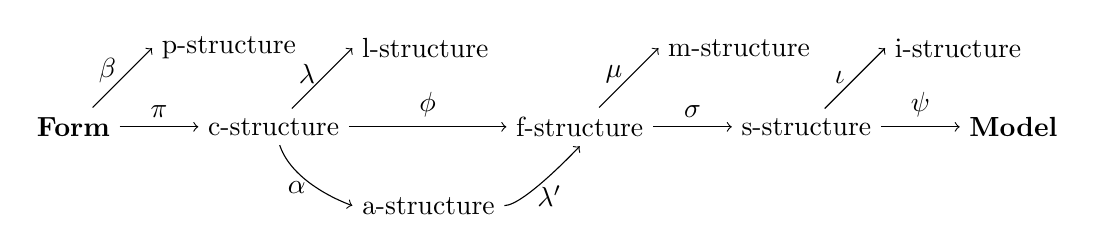
\begin{tikzpicture}
  \draw[->] (0,0) node(form)[anchor=east]{\textbf{Form}} -- ++(1,0) node(c-str)[anchor=west]{c-structure} node[pos=0.5,above]{$\pi$};
  \draw[->] (form) -- ++(1,1) node[anchor=west]{p-structure} node[pos=0.25,above]{$\beta$};
  
  \draw[->] (c-str.east) -- ++(2,0) node(f-str)[anchor=west]{f-structure} node[pos=0.5,above]{$\phi$};
  \draw[->] (c-str) -- ++(1,1) node[anchor=west]{l-structure} node[pos=0.25,above]{$\lambda$};
  
  \draw[->] (c-str) .. controls ++(0.25,-0.75) and ++(0,0) .. ++(1,-1) node(a-str)[anchor=west]{a-structure} node[pos=0.25,below]{$\alpha$};
  \draw[->] (a-str.east) .. controls ++(0.25,0) and ++(0,0) .. (f-str.south) node[pos=0.5,below]{$\lambda'$};
  
  \draw[->] (f-str.east) -- ++(1,0) node(s-str)[anchor=west]{s-structure} node[pos=0.5,above]{$\sigma$};
  \draw[->] (f-str) -- ++(1,1) node[anchor=west]{m-structure} node[pos=0.25,above]{$\mu$};
  
  \draw[->] (s-str.east) -- ++(1,0) node[anchor=west]{\textbf{Model}} node[pos=0.5,above]{$\psi$};
  \draw[->] (s-str) -- ++(1,1) node[anchor=west]{i-structure} node[pos=0.25,above]{$\iota$};
 \end{tikzpicture}
 }
 \zs
 
 To date, additional levels and projections that have been discussed
 and described in the LFG literature include the following (references to some of the proposals are given in parentheses; most have separate chapters in the handbook, which describe proposed representations in detail):
 
 \begin{itemize}
  \item argument structure (a-structure) \parencite{butt1997architecture}, see \citetv{chapters/Mapping};
  \item semantic structure (s-structure) \parencite{Dalrymple:Glue}, see \citetv{chapters/Glue};
  \item information structure (i-structure) \parencite{King1997,BK00,DN}, see \citetv{chapters/InformationStructure};
  \item prosodic structure (p-structure) \parencite{DM11,boegel2012}, see \citetv{chapters/Prosody};
  \item morphological / morphosyntactic structure (m-structure), see \parencite{butt-etal2004,sadler-nordlinger2004}, \citetv{chapters/Morphology};
  \item grammatical marking structure (g-structure) \parencite{falk06};
  \item l-structure, a level that represents complex categories of c-structure nodes in the approach of \citet{low:lov:20}: see \citetv{chapters/CoreConcepts}. 
 \end{itemize}

 \section{Conclusion}
 
In this chapter, I have described the main architectural notions of LFG -- the c- and f-structures. LFG can be viewed as incorporating the best features of constituent-structure-based (at c-structure) and dependency-based (at f-struc\-ture) frameworks, while avoiding their main drawbacks. Frameworks that use phrase structure as the only syntactic representation require additional mechanisms such as transformations, multiple dominance or separate linearization to properly capture word order variation and feature constraints; LFG manages to keep c-structure relatively simple due to the fact that all feature interactions are captured at f-structure, without referring to constituent structure positions. At the same time, the fact that f-structure does not directly refer to individual words or phrase structure nodes allows adequately capturing word order variation while keeping predicate-argument representations fairly uniform across languages.  I have also described how the core architecture may be extended to other projections beyond f-structure. Each of these modules captures a separate part of grammar (prosody, semantic structure, information structure, etc.) and has its own internal makeup. The modules are linked together using annotations of c-structure rules in the same way as f-structure is projected from c-structure. Hence, grammars in LFG are factorized into several distinct components, each of which is responsible for its own range of phenomena and largely operates according to its own principles, with c-structure serving as a ``hub'' tying all the components together.
 
\section*{Acknowledgements}

I am grateful to Mary Dalrymple for her insightful comments on this chapter and painstaking editorial work. I would also like to thank Tina Bögel for some comments on an earlier draft of the chapter. Finally, I am grateful to two anonymous reviewers for their attentive reading of the chapter and useful comments. This research has been supported by the Interdisciplinary Scientific and Educational School of Moscow University ``Preservation of the World Cultural and Historical Heritage''.

\sloppy
\printbibliography[heading=subbibliography,notkeyword=this] 
\end{document}
 
